
%%%%%%%%%%%%%%%%%%%%%%%%%%%%%%%%%%%%%%%%%%%%%%
\section{Installation}


%%%%%%%%%%%%%%%%%%%%%%
\subsection{Anode Plane Assemblies (APAs)}



%%%%%%%%%%%%%%%%%%%%%%
\subsection{Cathode Plane Assemblies (CPAs)}

%\subsection{Assembly  and Installation }

Individual CPA panels will be assembled off site and shipped to CERN in the horizontal position.  Each panel weights roughly 53 lbs and therefore can be lifted out of the shipping crate by hand and will not require and special fixtures.

The three CPA modules that made up a CPA panel will be placed on the floor and screwed/pinned together.   The crane then will be attached to the top of the CPA and it will be lifted to the vertical position.  

The load transfer from the crane hook to the installation rail still needs to be determined.  

Once two CPA planes are mounted they must be brought together within 1mm along their length.  (see thermal discussion in Section 7).  There will be two pins located on the side of the first CPA that will have to fit into a vertical slot on the side of the second CPA to lock them together in plane.  

The CPA plane may not hang vertically after being hung if the strap is not perfectly on center.  This can be corrected when the FC are mounted to a pair of CPA planes.  The connection points on the FC is fixed and therefore will tie the CPA’s together and force them to hang vertically because the assembly of the CPA planes and FC then becomes a two point support structure.  

During assembly the FC will be hung from the CPA.  In a worst case scenario the two FC will be mounted on one side of the CPA first which will cause the CPA to rotate 2.9'' due to the offset loading.  



%%%%%%%%%%%%%%%%%%%%%%
\subsection{Field Cage (FC)}

%\subsection{Assembly Sequence and QC Procedures}




%%%%%%%%%%%%%%%%%%%%%%
\subsection{Photon Detection System (PDS)}



%%%%%%%%%%%%%%%%%%%%%%
\subsection{Cold Electronics (CE)}
\label{subsec:ce_install}

Cold electronics will be mounted on the TPC and installed inside the cryostat.
Because access to the cold electronics is not possible after the cryostat is sealed,
a full complement of tests will be performed during the development stage and before the final installation
(Figure~\ref{fig:tpcce_CMBonAPA}).

\begin{cdrfigure}[The front end electronics as mounted on an APA]{tpcce_CMBonAPA}{The front end electronics as mounted on an APA.
  {\bf Top:} The front end electronics  is shown in the red circle.
  {\bf Bottom:} Cross section view.}
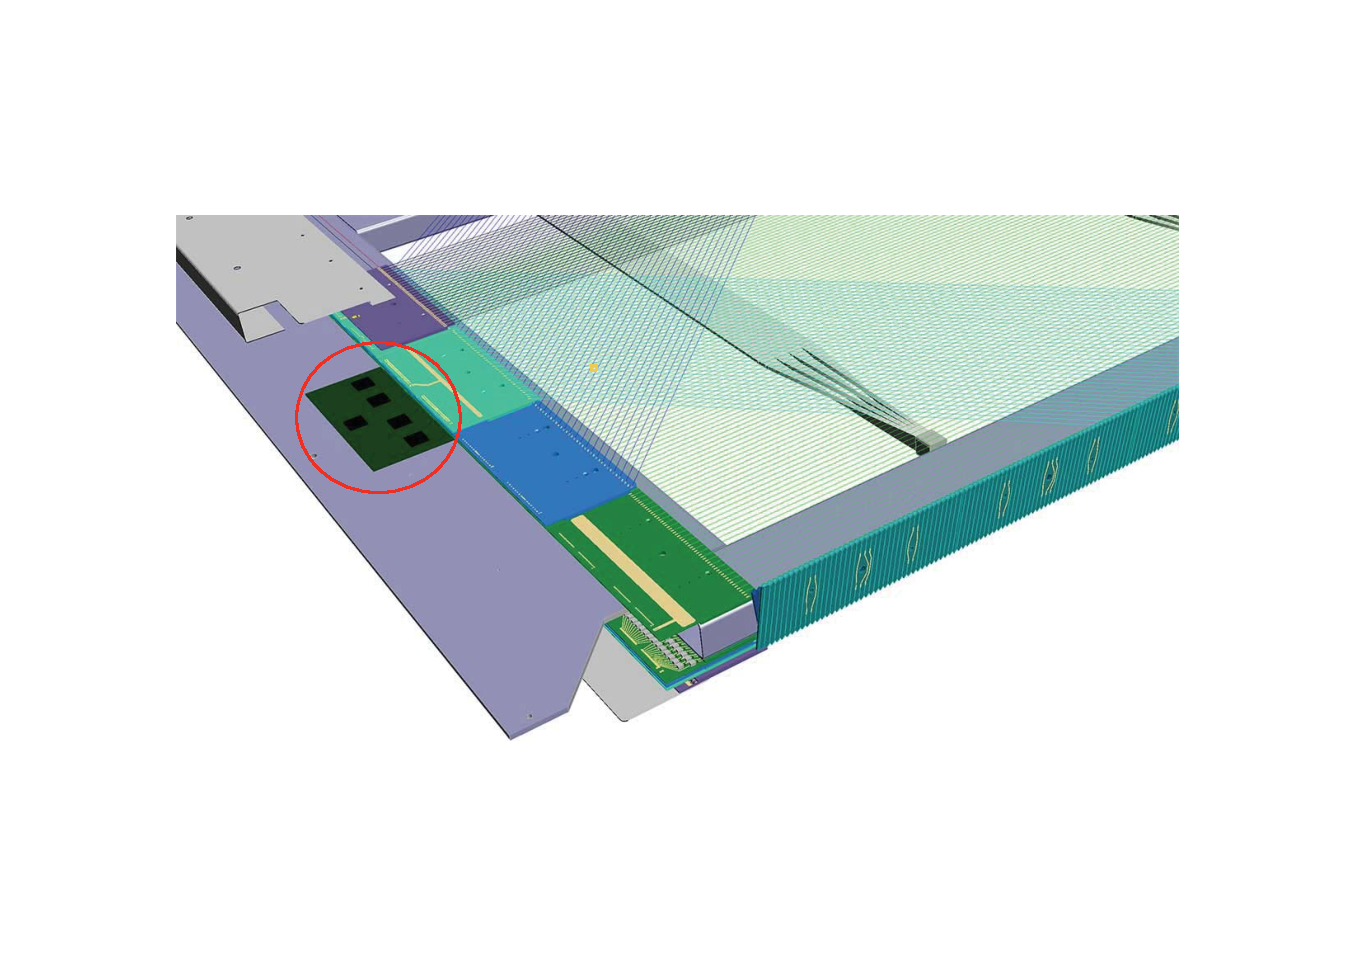
\includegraphics[width=1.00\linewidth]{tpcce_CMBonAPA_1.pdf}
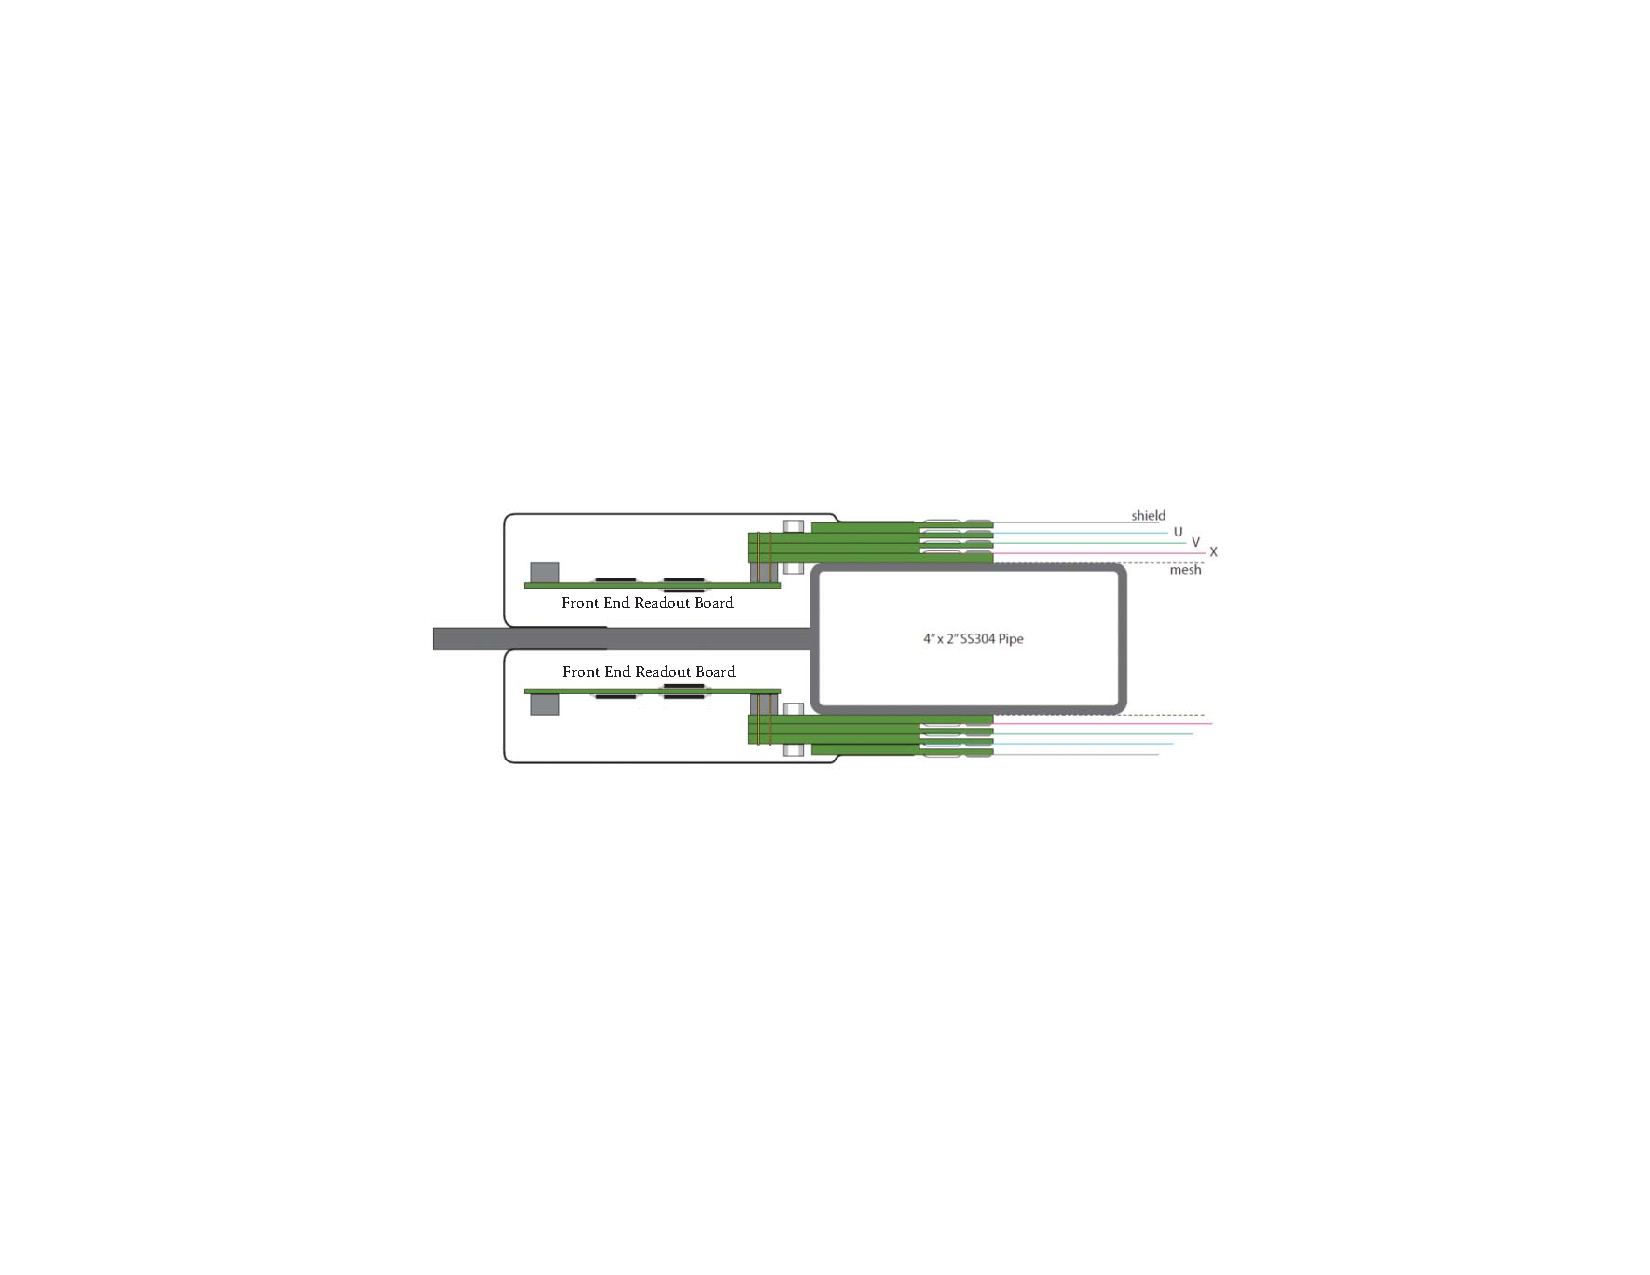
\includegraphics[width=1.00\linewidth]{tpcce_CMBonAPA_2.pdf}
\end{cdrfigure}

\fixme{Have two instances of this figure; we'll need to get rid of one. Anne}

%%%%%%%%%%%%%%%%%%%%%%%%%
\subsection{QC Procedures}

